\subsection{Depth of Investigation}
\begin{center}
\begin{tikzpicture}
      
    \newcommand\EMF{\mathcal{E}};
    \colorlet{Icol}{blue!50!black}
    \colorlet{Ccol}{orange!90!black}
    \colorlet{Rcol}{red}
    \colorlet{loopcol}{red!90!black!25}
    \colorlet{pluscol}{red!60!black}
    \colorlet{minuscol}{blue!60!black}
    \tikzstyle{EMF}=[battery1,l=$\EMF$];
    \tikzstyle{internal R}=[R,color=Rcol,Rcol,l=$r$,/tikz/circuitikz/bipoles/length=30pt];
    \tikzstyle{loop}=[->,red!90!black!25];
    \tikzstyle{loop label}=[loopcol,fill=white,scale=0.8,inner sep=1];
    \tikzstyle{thick R}=[R,color=Rcol,thick,Rcol,l=$R$];
    
    \begin{scope}[rotate=-90,transform shape]
      \fill[pattern = crosshatch dots,pattern color = brown!80!red] (0.0,-0.5) rectangle ++(6,11);
     % \node[rotate=90] at (0.25,1.5) {Surface};
      \draw (0,0)
      %to[R,color=Rcol,thick,l={{{{\rotatebox[origin=c]{90}{$R_{c2}$}}}}}] (6,9) 
      %to[R,color=Rcol,thick,l={{{{\rotatebox[origin=c]{90}{$R$}}}}}] (6,0) 
      %to[R,color=Rcol,thick,l={{{{\rotatebox[origin=c]{90}{$R_{c1}$}}}}}] (0,0) 
      to [ammeter, color=black] (0,9);
      \node[rotate=90,above] at (0,9) {$B$};
      \node[rotate=90,above] at (0,0) {$A$};
 
     % \node[rotate=90] at (0,4) {$\Delta V$};
        %  \draw[->,red] (0.5, 2.15) --++ (1.2,0) node[midway,above=1] {current $I$};
        %  \draw[->,red] (0.5,-0.15) --++ (1.2,0) node[midway,below=1] {electron flow};
      \end{scope}
    %   \draw[-,color=black] (2,-0.8) -- (2,1.2);
    %   \draw[-,color=black] (2,1.2) -- node[above] {$\Delta$ U} (5,1.2);
    %   \draw[-,color=black] (5,1.2) -- (5,-0.8);
      \draw[<->,color=blue,line width=0.75mm] (3,1.5) -- (0.0,1.5) node[midway,below] {$x$};
      \draw[<->,color=blue,line width=0.75mm] (3.0,1.5) -- (9.0,1.5) node[midway,below] {$x-L$};
      \draw[<->,color=blue,line width=0.75mm] (3.0,1.5) -- (9.0,1.5) node[midway,below] {$x-L$};
      \draw[<->,color=blue,line width=0.75mm] (0.0,0.9) -- (9.0,0.9) node[midway,below] {$L$};
      \draw[-,color=black,dashed,,line width=0.75mm] (3.0,0.0) -- (3.0,-6);
      \draw[-,color=black,line width=0.75mm] (0.0,0.0) -- (3.0,-4) node[midway,sloped,above] {$r_1$};
      \draw[-,color=black,line width=0.75mm] (0.0,0.0) -- (3.0,-4) node[midway,sloped,above] {$r_1$};
      \draw[-,color=black,line width=0.75mm] (9,0) -- (3.0,-4) node[midway,sloped,above] {$r_2$};
      \draw[->,color=black,line width=1.0mm] (2.5,-2.1) -- (3.5,-2.1) node[left,above] {$J_x$};
      \draw[->,color=black,line width=1.0mm] (2.5,-3.1) -- (3.5,-3.1) node[left,above] {$J_x$};
      \draw[->,color=black,line width=1.0mm] (2.5,-4.1) -- (3.5,-4.1) node[left,above] {$J_x$};
      \draw[->,color=black,line width=1.0mm] (2.5,-5.1) -- (3.5,-5.1) node[left,above] {$J_x$};
    %   \node[above] at (2,1.2) {$M$};
    %   \node[above] at (5,1.2) {$N$};
  \end{tikzpicture}
\end{center}
(\textit{tricky}) In this exercise we would like to approximate which depth interval the resistivity method is sensitive to. We already understand intuitively that a larger electrode spacing between A and B increases the depth penetration. Here we aim to do it quantitatively. For this we consider a vertical plane located at distance $x$ away from electrode A, and calculate how much of the current flow density crosses that plane. This means we would like to calculate $J_x(z)$. From the lecture we know that:

$$
\vec{j} = \sigma \vec{E} = \sigma \nabla V \rightarrow J_x = -\frac{I}{2\pi} \frac{\partial }{\partial x} \left(\frac{1}{r_1} - \frac{1}{r_2}\right )
$$
Adopting the coordinate system from the Figure above we choose $r_1 =\sqrt{x^2+y^2+z^2}$ with z point along depth and y into the plane. First calculate $J_x$ for any point P, then show that 
$$
J_x (x=L/2) = \frac{I}{2\pi}\frac{L}{(z^2+y^2+\frac{L^2}{4})^{3/2}}
$$
at the center point. Sketch this function roughly on paper for a fixed L. Now consider a fixed layer at constant depth $z$. How does $J_x$ change as $L$ is varied? Show that $J_x(x=L/2,z)$ has a maximum at $L=\sqrt{2}{z}$. This shows that depth penetration increases as we increase the distance between the current electrodes A and B. Still, most of the current flow will be near the surface. In order to define a depth of investigation we will need to apply some thresholding and include placement of the M,N electrodes. This varies from array to array.
\ifanswers
    \begin{tcolorbox}[enhanced jigsaw,breakable,pad at break*=1mm,
    colback=blue!5!white,colframe=babyblueeyes,title=Solutions,
    watermark color=white]
   
   
 
      Calculation of the derivative is:
      \begin{eqnarray*}
        &-\frac{I}{2\pi} \frac{\partial }{\partial x} \left(\frac{1}{r_1} - \frac{1}{r_2}\right) =  \\
        &-\frac{I}{2\pi} \frac{\partial }{\partial x} \left(\frac{1}{\sqrt{x^2+y^2+z^2}} - \frac{1}{\sqrt{(x-L)^2+y^2+z^2}}\right)= \\
        &\frac{I}{4\pi}  \left(\frac{2x}{(x^2+y^2+z^2)^{3/2}} - \frac{2(x-L)}{((x-L)^2+y^2+z^2)^{3/2}}\right)= \\
        &\frac{I}{2\pi}  \left(\frac{x}{(x^2+y^2+z^2)^{3/2}} - \frac{(x-L)}{((x-L)^2+y^2+z^2)^{3/2}}\right)
     \end{eqnarray*}
     Now consider this for the center at $x=\frac{L}{2}$ where $r_1 = r_2 = \sqrt{L^2/4+y^2+z^2}$:
     \begin{eqnarray*}
      &J_x(x=L/2) =   \\
      & \frac{I}{2\pi}\left(\frac{L/2}{(L^2/4+y^2+z^2)^{3/2}} + \frac{(L/2)}{(L^2/4+y^2+z^2)^{3/2}}\right) = \\
      &\frac{I}{2\pi}  \left(\frac{L}{(L^2/4+y^2+z^2)^{3/2}}\right)
     \end{eqnarray*}
     \begin{center}
     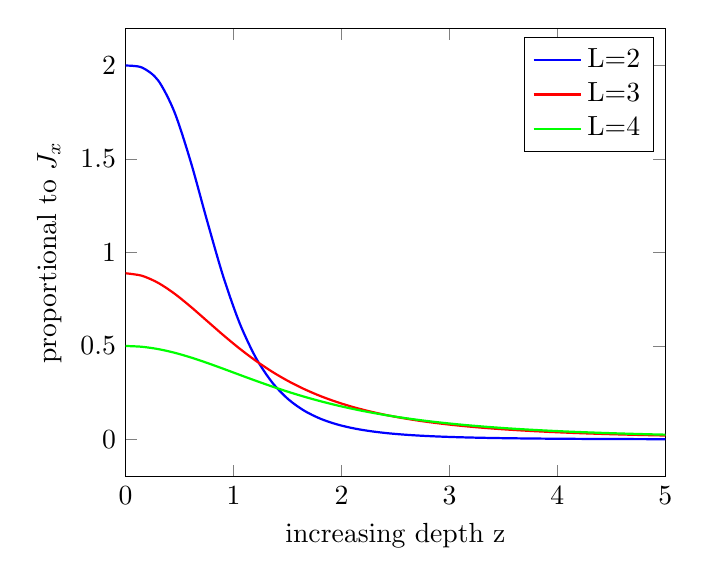
\begin{tikzpicture}
     \begin{axis}[
      xmin = 0, xmax = 5,xlabel=increasing depth z,
      ylabel={proportional to $J_x$}]
      \addplot[
          domain = 0:30,
          samples = 200,
          smooth,
          thick,
          blue,
      ] {2/(x^3+2*2/4)^(3/2)};
      \addplot[
        domain = 0:30,
        samples = 200,
        smooth,
        thick,
        red,
    ] {3/((x^2+3*3/4)^(3/2))};
    \addplot[
      domain = 0:30,
      samples = 200,
      smooth,
      thick,
      green,
     ] {4/((x^2+4*4/4)^(3/2))};
  \legend{L=2,L=3,L=4}
  \end{axis}
\end{tikzpicture}
\end{center}
Next we calculate the derivative with respect to $L$ (at x=L/2 and y=0):
\begin{eqnarray*}
  \frac{\partial}{\partial L}\left(\frac{L}{(L^2/4+z^2)^{3/2}}\right) = 0 \\
  (L^2/4+z^2)^{-3/2} -\frac{3}{2}L (L^2/4+z^2)^{-5/2}L/2 = 0 \\
  1 -\frac{3}{4}L^2 (L^2/4+z^2)^{-1} = 0 \\
  \rightarrow L^2/4+z^2 = \frac{3}{4}L^2 \\
  \rightarrow -L^2/2+z^2 = 0 \\
  \rightarrow L^2 = 2 z^2 \\
  \rightarrow L = \sqrt{2} z \\
\end{eqnarray*}

\begin{center}
  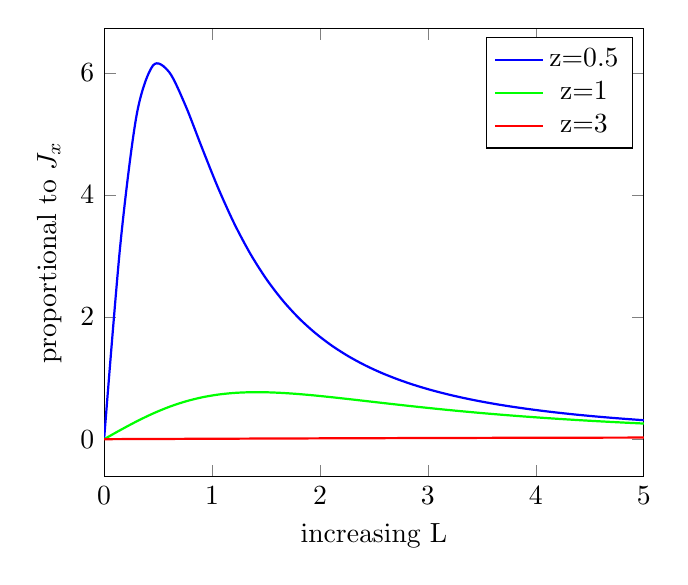
\begin{tikzpicture}
  \begin{axis}[
   xmin = 0, xmax = 5,xlabel=increasing L,
   ylabel={proportional to $J_x$}]
   \addplot[
       domain = 0:30,
       samples = 200,
       smooth,
       thick,
       blue,
   ] {x/(0.5^3+x*x/4)^(3/2)};
   \addplot[
    domain = 0:30,
    samples = 200,
    smooth,
    thick,
    green,
] {x/(1^3+x*x/4)^(3/2)};
\addplot[
  domain = 0:30,
  samples = 200,
  smooth,
  thick,
  red,
] {x/(3^3+x*x/4)^(3/2)};
 \legend{z=0.5,z=1,z=3}
\end{axis}
\end{tikzpicture}
Normalized in Telford chapter 8.
\end{center}

\end{tcolorbox}

\fi
